\documentclass{beamer}
\usepackage{graphicx}
\usepackage{array}
\title{Growth Monitoring Unit (GMU) and TinyML Model}
\author{}
\date{}

\begin{document}

\frame{\titlepage}

\begin{frame}{GMU Rail System}
    \begin{itemize}
        \item Provides precise linear movement for the Growth Monitoring Unit (GMU)
        \item Stepper motors rotate pulleys $\rightarrow$ belt moves carriage $\rightarrow$ GMU slides along rail
        \item Ensures accurate, repeatable, low-maintenance motion
        \item Components: linear rail, carriage block, belt \& pulley, stepper motors, idlers, tensioners, mounting brackets
        \item Enables automated plant imaging for TinyML-based growth stage detection
    \end{itemize}
\end{frame}

\begin{frame}{Image: Model of GMU Rail System}
    \begin{figure}
        \centering
        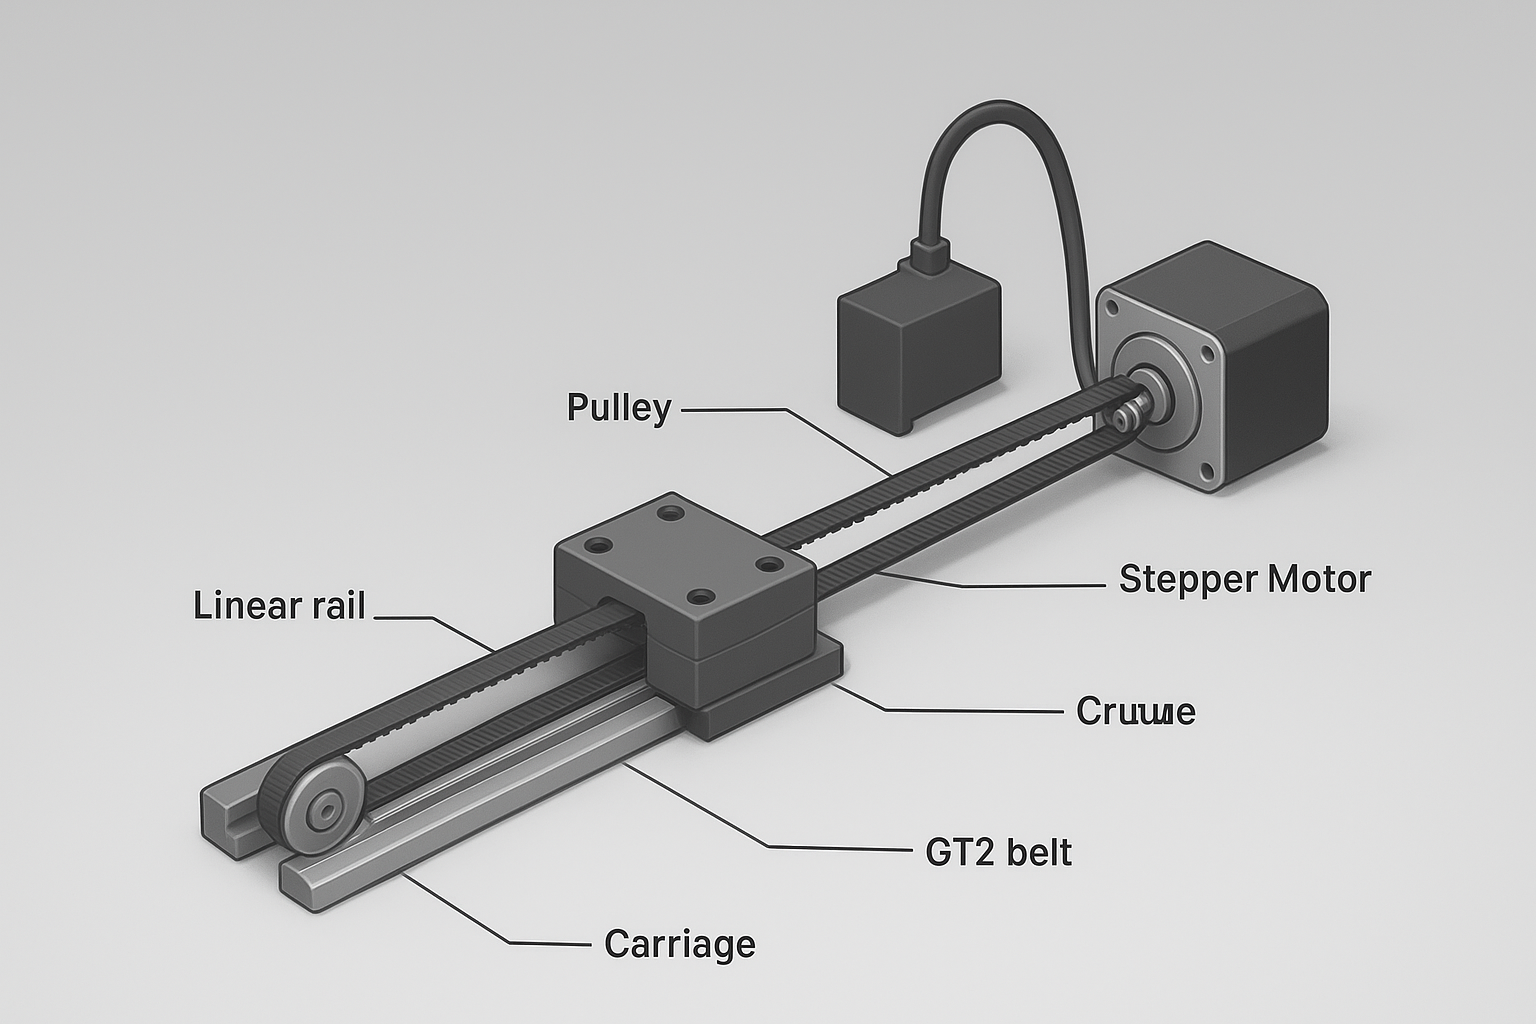
\includegraphics[width=0.8\textwidth]{railmodel.png}
        \caption{Model of GMU Rail System}
    \end{figure}
\end{frame}

\begin{frame}{Sensing and Motion Subsystem}
    \begin{itemize}
        \item Components:
        \begin{itemize}
            \item ESP32 CAM
            \item Environmental sensors
            \item User app, cloud server
            \item ESP32 main controller
            \item Mobile carriage, motor driver, stepper motor, linear rail system
        \end{itemize}
        \item Enables automatic plant growth monitoring
    \end{itemize}
\end{frame}

\begin{frame}{Image: GMU Rail System Architecture}
    \begin{figure}
        \centering
        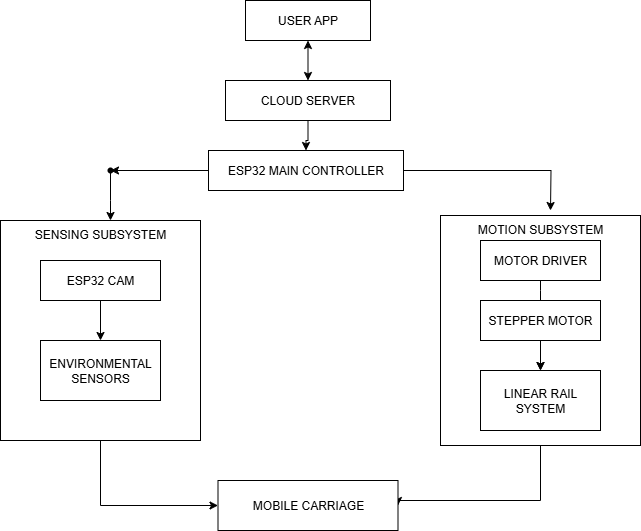
\includegraphics[width=0.8\textwidth]{rail3.drawio.png}
        \caption{GMU Rail System Architecture}
    \end{figure}
\end{frame}

\begin{frame}{TinyML Model: Overview}
    \begin{itemize}
        \item CNN-based model optimized for ESP32 deployment
        \item Lightweight, real-time predictions (90–95\% accuracy)
        \item Output: stage label $\pm$ confidence, can trigger automated actions
        \item Classifies plant growth stages: Germination $\rightarrow$ Sprout $\rightarrow$ Early Growth $\rightarrow$ Mature
        \item First level output of sprout stage determined
    \end{itemize}
\end{frame}

\begin{frame}{Image: CNN Model Architecture}
    \begin{figure}
        \centering
        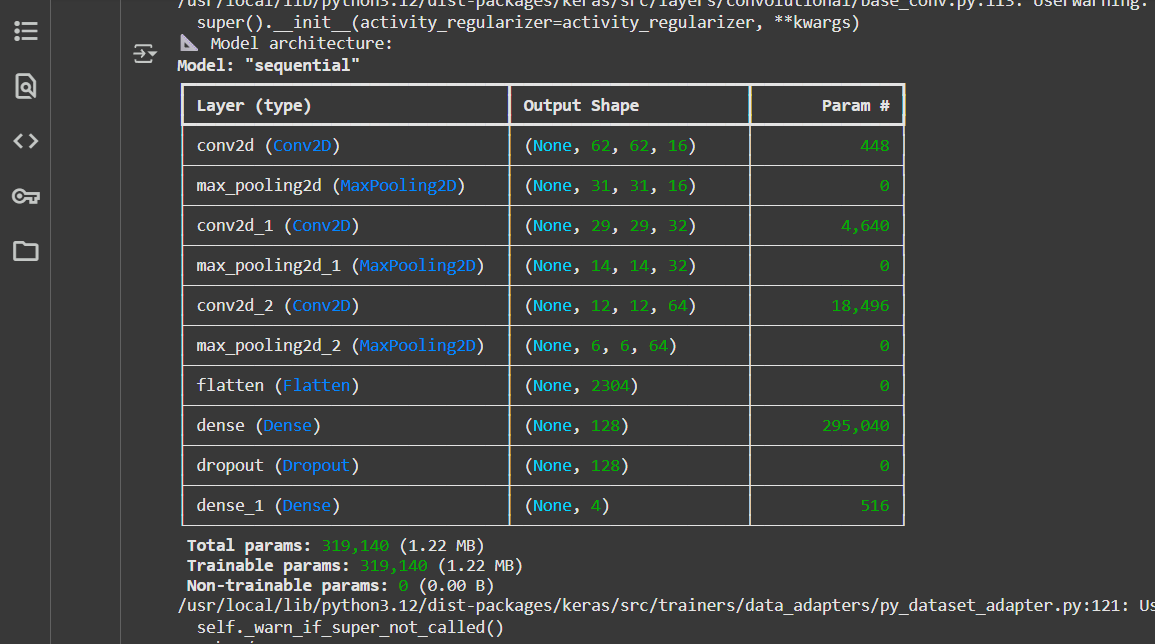
\includegraphics[width=0.8\textwidth]{modelrender.png}
        \caption{CNN Model Architecture}
    \end{figure}
\end{frame}

\begin{frame}{Deployment and Results}
    \begin{itemize}
        \item Model saved as \texttt{sprout_detector.h5} $\rightarrow$ converted to \texttt{sprout_detector.tflite} for ESP32-CAM
        \item Accuracy \& Loss graphs (side-by-side); see attached figures
        \item Confusion matrix, example inference outputs highlight classification performance
    \end{itemize}
\end{frame}

\begin{frame}{Image: Accuracy, Loss Graphs, and Confusion Matrix}
    \begin{figure}
        \centering
        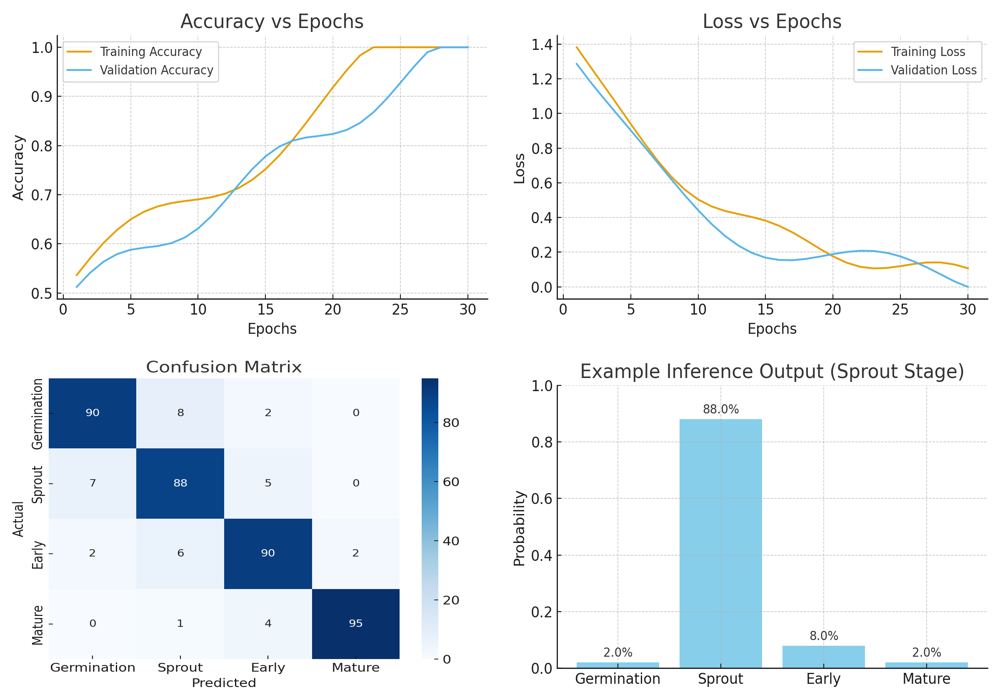
\includegraphics[width=0.8\textwidth]{tinyml_results_slide.png}
        \caption{Accuracy, Loss Graphs, and Confusion Matrix}
    \end{figure}
\end{frame}

\begin{frame}{Component Price and Count}
    \centering
    \resizebox{\textwidth}{!}{%
        \begin{tabular}{|>{\raggedright}p{5cm}|r|c|r|}
            \hline
            \textbf{Component name} & \textbf{Price of single component} & \textbf{Count} & \textbf{Total price} \\
            \hline
            ESPCAM & 750 & 1 & 750 \\
            ESPCAM Programmer & 91 & 1 & 91 \\
            SD Card & 480 & 1 & 480 \\
            17HS3401S NEMA17 Stepper Motor & 544 & 2 & 1088 \\
            DRV8825 stepper driver module & 94 & 2 & 188 \\
            GT2 6mm Belt Width 20 Teeth 5mm Bore Timing Pulley & 42 & 2 & 84 \\
            Linear Rail & 1504 & 3 & 4512 \\
            Limit switch & 23 & 2 & 46 \\
            Belt tensioner & 52 & 1 & 52 \\
            Rail mounting brackets & 69 & 4 & 276 \\
            \hline
            \multicolumn{3}{|r|}{\textbf{Total}} & \textbf{7567} \\
            \hline
        \end{tabular}
        }
\end{frame}


\end{document}
